\documentclass[12pt]{article}
\usepackage[letterpaper, hmargin=0.75in, vmargin=0.75in]{geometry}
\usepackage{float}
\usepackage{url}
\usepackage{graphicx}
\usepackage{tikz}
\usepackage{verbatimbox}

\usetikzlibrary{arrows,automata,shapes}
\tikzstyle{block} = [rectangle, draw, fill=blue!20,
    text width=5em, text centered, rounded corners, minimum height=2em]

\title{SE465-001\\Assignment 2}
\author{Kevin Carruthers (20463098), {\tt KevinJames@thekev.in}}
\date{February 23, 2015}

\begin{document}

\maketitle

\section*{Question 1}
Yes. Assuming a graph is acyclical, it must be possible to covere each path in the graph with some combination of prime paths. Since PPC covers all such paths, and CPC simply requires all paths are covered, it must be the case that PPC subsumes CPC in this case.

\section*{Question 2}
\paragraph{Test Case 1 Memory Problem.} The problem here is that our delete function does not free memory associated with \ttfamily{node->str}\rmfamily{}. This issue was fixed by adding a call to \ttfamily{free()}\rmfamily{}. The following valgrind output was observed:
\begin{verbnobox}[\scriptsize]
==18848== Memcheck, a memory error detector
==18848== Copyright (C) 2002-2013, and GNU GPL'd, by Julian Seward et al.
==18848== Using Valgrind-3.10.0 and LibVEX; rerun with -h for copyright info
==18848== Command: sll_buggy
==18848==
==18848==
==18848== HEAP SUMMARY:
==18848==     in use at exit: 9 bytes in 1 blocks
==18848==   total heap usage: 5 allocs, 4 frees, 67 bytes allocated
==18848==
==18848== 9 bytes in 1 blocks are definitely lost in loss record 1 of 1
==18848==    at 0x4C2B41E: realloc (in /usr/lib64/valgrind/vgpreload_memcheck-amd64-linux.so)
==18848==    by 0x400990: fgets_enhanced (sll_buggy.c:47)
==18848==    by 0x40125A: main (sll_buggy.c:279)
==18848==
==18848== LEAK SUMMARY:
==18848==    definitely lost: 9 bytes in 1 blocks
==18848==    indirectly lost: 0 bytes in 0 blocks
==18848==      possibly lost: 0 bytes in 0 blocks
==18848==    still reachable: 0 bytes in 0 blocks
==18848==         suppressed: 0 bytes in 0 blocks
==18848==
==18848== For counts of detected and suppressed errors, rerun with: -v
==18848== ERROR SUMMARY: 1 errors from 1 contexts (suppressed: 0 from 0)
\end{verbnobox}

\paragraph{Test Case 2 Memory Problem.} The problem here is that \ttfamily{p}\rmfamily{} is not set back to \ttfamily{NULL}\rmfamily{} after deleting all entries in the list. This issue was fixed by adding \ttfamily{p = NULL;}\rmfamily{} to the \ttfamily{delete\_all()}\rmfamily{} function. The following valgrind output was observed:
\begin{verbnobox}[\scriptsize]
==20711== Memcheck, a memory error detector
==20711== Copyright (C) 2002-2013, and GNU GPL'd, by Julian Seward et al.
==20711== Using Valgrind-3.10.0 and LibVEX; rerun with -h for copyright info
==20711== Command: sll_buggy
==20711==
==20711== Invalid read of size 8
==20711==    at 0x400B7E: delete_all (sll_fixed.c:106)
==20711==    by 0x4013DB: main (sll_fixed.c:327)
==20711==  Address 0x51dd0a0 is 16 bytes inside a block of size 24 free'd
==20711==    at 0x4C2A37C: free (in /usr/lib64/valgrind/vgpreload_memcheck-amd64-linux.so)
==20711==    by 0x400B9D: delete_all (sll_fixed.c:109)
==20711==    by 0x401391: main (sll_fixed.c:314)
==20711==
==20711== Invalid read of size 8
==20711==    at 0x400B8A: delete_all (sll_fixed.c:108)
==20711==    by 0x4013DB: main (sll_fixed.c:327)
==20711==  Address 0x51dd090 is 0 bytes inside a block of size 24 free'd
==20711==    at 0x4C2A37C: free (in /usr/lib64/valgrind/vgpreload_memcheck-amd64-linux.so)
==20711==    by 0x400B9D: delete_all (sll_fixed.c:109)
==20711==    by 0x401391: main (sll_fixed.c:314)
==20711==
==20711== Invalid free() / delete / delete[] / realloc()
==20711==    at 0x4C2A37C: free (in /usr/lib64/valgrind/vgpreload_memcheck-amd64-linux.so)
==20711==    by 0x400B91: delete_all (sll_fixed.c:108)
==20711==    by 0x4013DB: main (sll_fixed.c:327)
==20711==  Address 0x51dd040 is 0 bytes inside a block of size 5 free'd
==20711==    at 0x4C2A37C: free (in /usr/lib64/valgrind/vgpreload_memcheck-amd64-linux.so)
==20711==    by 0x400B91: delete_all (sll_fixed.c:108)
==20711==    by 0x401391: main (sll_fixed.c:314)
==20711==
==20711== Invalid free() / delete / delete[] / realloc()
==20711==    at 0x4C2A37C: free (in /usr/lib64/valgrind/vgpreload_memcheck-amd64-linux.so)
==20711==    by 0x400B9D: delete_all (sll_fixed.c:109)
==20711==    by 0x4013DB: main (sll_fixed.c:327)
==20711==  Address 0x51dd090 is 0 bytes inside a block of size 24 free'd
==20711==    at 0x4C2A37C: free (in /usr/lib64/valgrind/vgpreload_memcheck-amd64-linux.so)
==20711==    by 0x400B9D: delete_all (sll_fixed.c:109)
==20711==    by 0x401391: main (sll_fixed.c:314)
==20711==
==20711==
==20711== HEAP SUMMARY:
==20711==     in use at exit: 0 bytes in 0 blocks
==20711==   total heap usage: 10 allocs, 16 frees, 119 bytes allocated
==20711==
==20711== All heap blocks were freed -- no leaks are possible
==20711==
==20711== For counts of detected and suppressed errors, rerun with: -v
==20711== ERROR SUMMARY: 12 errors from 4 contexts (suppressed: 0 from 0)
\end{verbnobox}

\paragraph{Test Case 3 Memory Problem.} Here is a test case for the new bug:
\begin{verbatim}
> i
> 100
> Tom
> i
> 111
> Mary
> p
> x
\end{verbatim}
This bug is a printing issue: the print format is ``\ttfamily{The elements are :>  -> 100, Tom -> 111, Mary}\rmfamily{}'' when it should clearly be ``\ttfamily{The elements are :> 100, Tom -> 111, Mary}\rmfamily{}'' (ie. without implying the first node is \ttfamily{NULL}\rmfamily{} or empty. This issue was fixed by modifying the logic in \ttfamily{display()}\rmfamily{} to ensure the arrow was only drawn when necessary (ie. after the first element).

\section*{Question 3}
Mutant 1 is:
\begin{verbatim}
int list_has_cycle(NODE *list) {
    NODE *fast=list;
    while(1) {
        if(!(fast=fast->next)) return 0;
        if(fast==fast) return 1;
        if(!(fast=fast->next)) return 0;
        if(fast==list) return 1;
        list=list->next;
    }
    return 0;
}
\end{verbatim}
and we can kill it with the following test input:
\begin{verbatim}
void test() {
    NODE *a, *b, *c;

    a->next = b;
    b->next = c;
    c->next = NULL;

    printf("Test Result: %d\n", list_has_cycle(a));
}
\end{verbatim}

Expected output is \ttfamily{Test Result: 0}\rmfamily{}.

Mutant 2 is:
\begin{verbatim}
int list_has_cycle(NODE *list) {
    NODE *fast=list;
    while(1) {
        if(!(fast=fast->next)) return 0;
        if(fast==list) return 1;
        if(!(fast=fast->next)) return 0;
        if(fast==list) return 1;
        list=list->next->next;
    }
    return 0;
}
\end{verbatim}
and we can kill it with the following test input:
\begin{verbatim}
void test() {
    NODE *a, *b, *c;

    a->next = b;
    b->next = c;
    c->next = a;

    printf("Test Result: %d\n", list_has_cycle(a));
}
\end{verbatim}

Expected output is \ttfamily{Test Result: 1}\rmfamily{}.

\section*{Question 4}
\paragraph{(a)}
\begin{figure*}[htb]
  \begin{center}
    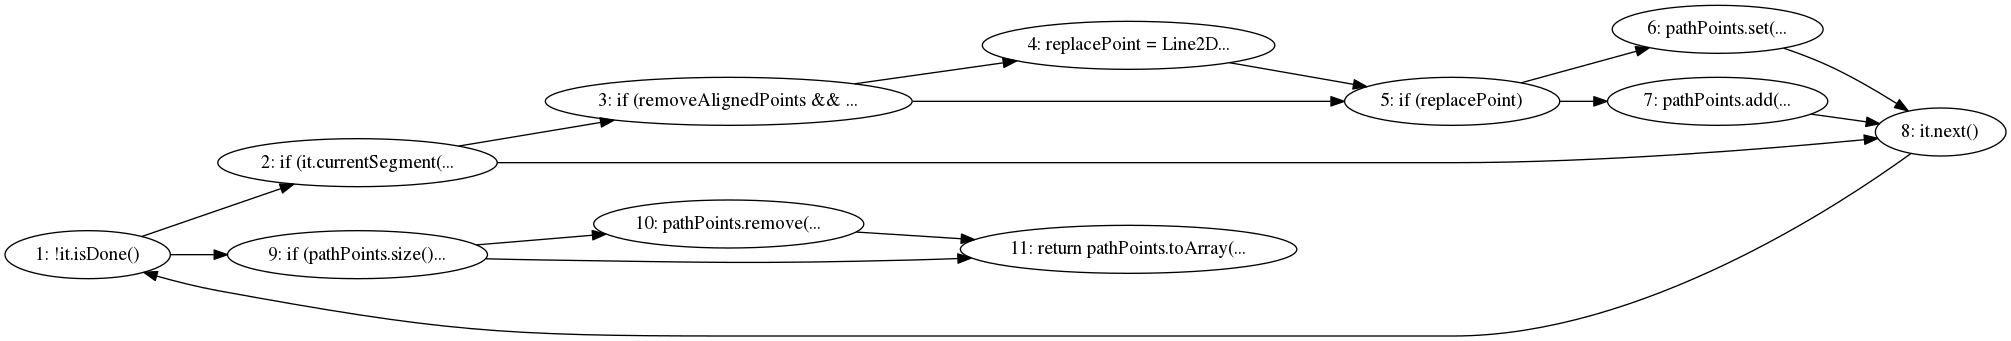
\includegraphics[width=\textwidth]{blockCFG}
  \end{center}
  \caption{Block CFG}
\end{figure*}

\begin{figure*}[htb]
  \begin{center}
    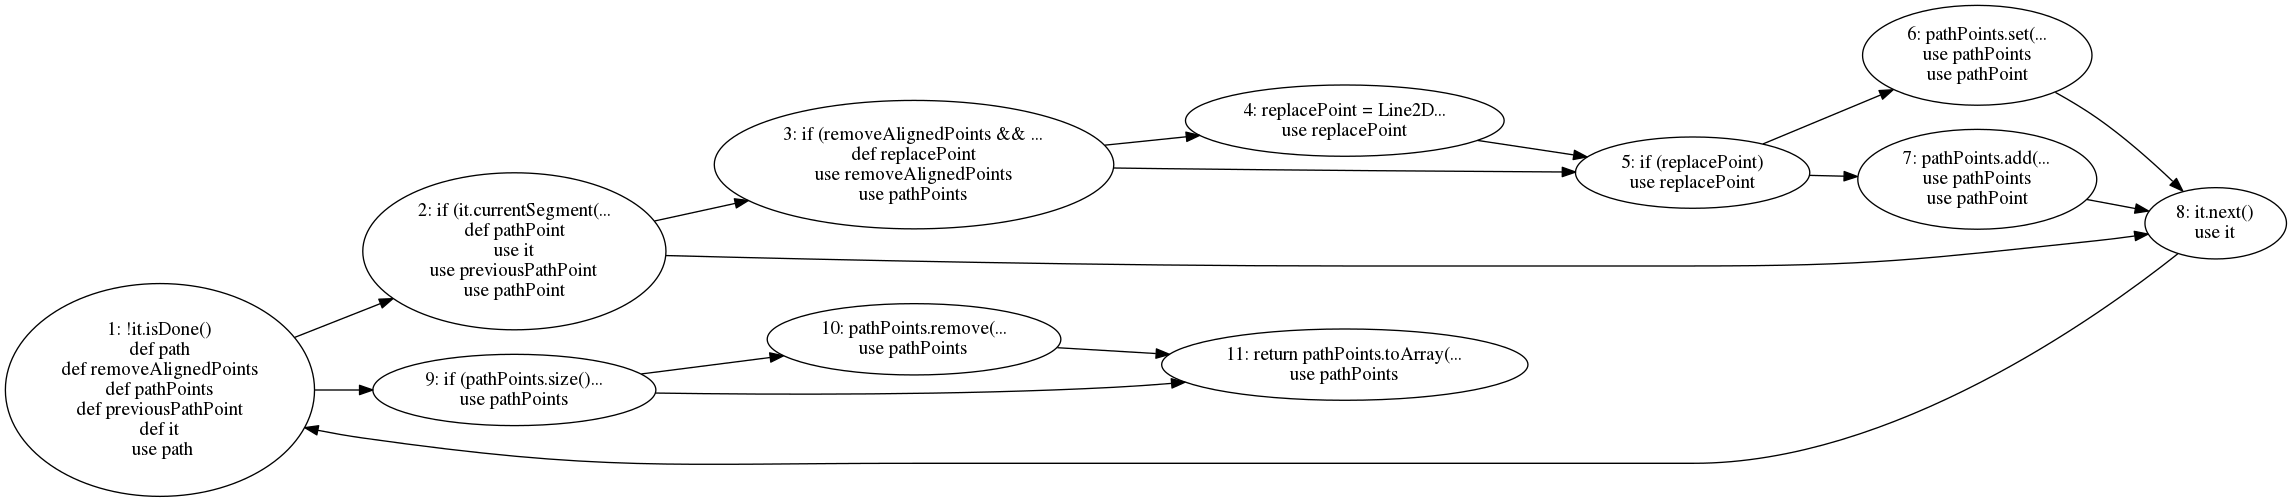
\includegraphics[width=\textwidth]{defuseCFG}
  \end{center}
  \caption{Def-Use CFG}
\end{figure*}

\paragraph{(b)} PPC requirements:
\begin{itemize}
\item $[1, 2, 3, 4, 5, 6, 8, 1, 9, 10, 11]$
\item $[1, 2, 3, 4, 5, 7, 8, 1, 9, 10, 11]$
\item $[1, 2, 8, 1, 9, 10, 11]$
\item $[1, 9, 10, 11]$
\item $[1, 9, 11]$.
\end{itemize}

\paragraph{(c)} To achieve ADC coverage, we may simply cover $[1, 2, 3]$. This covers each of our def blocks. For AUC coverage, we must cover $[1, 2, 3, 4, 5, 6, 8, 1, 9, 10, 11]$ as well as $[1, 2, 3, 5, 7]$. This ensure all use blocks are covered.

\paragraph{(d)} Strengths and Weaknesses: ADC and AUC coverage will ensure that all variables are properly used after they are declared, etc. PPC coverage will ensure that all logical decision are valid. In this case, PPC subsumes ADC and AUC, and is thus a much stronger form of coverage. The added test cases, ie. covering more potential decisions within the program, is worth the additional two test cases as we will have the potential to discover more issues in our code.

\paragraph{(e)} Test Cases:
\begin{itemize}
\item To cover path $[1, 2, 3, 4, 5, 6, 8, 1, 9, 11]$ we must have a path with a single item not set to \ttfamily{SEG\_CLOSE}\rmfamily{}, removedAlignedPoints set to \ttfamily{true}\rmfamily{} and replacePoint set to true (ie. the distance must be less than $0.0001$). Our output should be a single point.
\item To cover path $[1, 2, 3, 4, 5, 7, 8, 1, 9, 11]$ we must have a path with a single item not set to \ttfamily{SEG\_CLOSE}\rmfamily{}, removedAlignedPoints set to \ttfamily{true}\rmfamily{} and replacePoint set to \ttfamily{false}\rmfamily{} (ie. the distance must be greater than or equal to $0.0001$). Our output should be a single point.
\item To cover path $[1, 2, 8, 1, 9, 11]$ we must have a path with a single item set to \ttfamily{SEG\_CLOSE}\rmfamily{}. Our output should be a single point.
\item To cover path $[\dots, 1, 9, 10, 11]$, we must have at least two items in our path and removeAlignedPoints set to \ttfamily{false}\rmfamily{}. Furthermore, the first and last items in the path should be equal. We should expect output of size one less than the input length of our path.
\item To cover path $[1, 9, 11]$, we must have at least two items in our path and removeAlignedPoints set to \ttfamily{false}\rmfamily{}. Furthermore, the first and last items in the path should not be equal. We should expect output of size equal to the input length of our path.
\end{itemize}

\end{document}
